\documentclass[a4paper]{report}
\usepackage[utf8]{inputenc}
\usepackage{float}
\usepackage[pdftex]{graphicx}
\usepackage{amsmath}
\usepackage[pdftex]{hyperref}
\usepackage{tabularx}
\usepackage{xcolor} % for \textcolor
\usepackage{siunitx} % for SI units
\usepackage{amsfonts} % for things like \mathbb
\usepackage{booktabs} % for \toprule,...
\usepackage{subcaption} % for \captionsetup
\usepackage{adjustbox} % for \adjincludegraphics
\usepackage{multirow} % for multirow tables
\usepackage[backend=biber, style=ieee, sorting=none, natbib=true, mincitenames=1, maxcitenames=2]{biblatex} % biblatex config like in the dissertation
\bibliography{refs}
\usepackage[inkscapeformat=pdf]{svg} % svg support

\DeclareGraphicsExtensions{.pdf,.jpeg,.png,.PNG}

% \DeclareUnicodeCharacter{2212}{-} % fix error LaTeX Error: Unicode character − (U+2212)

\title{Reinforcement Learning for Human Intention Anticipation in Collaborative Tasks}
\author{Pedro Miguel Loureiro Amaral}
\date{July 15, 2024}

\begin{document}

\maketitle

\renewcommand\thesection{\arabic{section}}

\section{Introduction}
\section{Experimental Setup}
\label{section:system_architecture}

The work described in this dissertation is part of the AUGMANITY project\footnote{AUGMANITY website: \url{https://www.augmanity.pt}} that aims to develop technologies to support people operating in industrial environments. The experimental setup comprises the integration of both hardware and software components in a prototype collaborative cell (LARCC) at the Laboratory for Automation and Robotics (LAR) located in the Department of Mechanical Engineering at the University of Aveiro, as illustrated in \autoref{fig:LARCC}. The LARCC is equipped with a UR10e collaborative robot and multimodal sensor devices, including three LiDAR Velodyne sensors and four Orbbec 3D cameras distributed throughout the work volume. The software architecture is built upon the ROS middleware \cite{Quigley2009}, providing a robust framework for communication and coordination among the various components. In this context, this section provides a description of the materials used during this study and the methodological approaches followed to face the key challenges. 

\begin{figure}[ht]
    \centering
    \includegraphics[width=0.75\columnwidth]{figs/LARCC_prototype.pdf}
    \caption{Prototype collaborative cell LARCC}
    \label{fig:LARCC}
\end{figure}

\if{0}
\begin{figure}[!ht]
\centerline{\includegraphics[width=0.9\textwidth, trim={0 5cm 0 0}, clip]{figs/setup2.jpg}}
\caption[setup]{LAR hardware setup}
\label{fig:LARCC}
\end{figure}
\fi

\subsection{Robot Operating System (ROS)}

ROS\cite{ROS2}\footnote{ROS 1 documentation: \url{https://wiki.ros.org}}\footnote{ROS 2 documentation: \url{https://docs.ros.org/en/humble}} is an open-source collection of tools and software libraries used to develop a robotics application and, in this work, it is used to establish communication throughout all of the infrastructure. ROS was chosen due to the hardware abstraction it offers given that it contains driver packages to deal with some hardware devices, allowing for easier communication with the robot and the cameras. Other relevant features include:
\begin{itemize}
    \item \textbf{message broker}: every process in the project is a node in the ROS network and communicates with the other nodes mainly through topics (asynchronous publish/subscribe streaming of data) or services (synchronous RPC-style communication).
    \item \textbf{code reuse}: executables and packages are written to be as independent as possible, making the developer able to reuse them in another project.
    \item \textbf{rich ecosystem}: there are several open-source packages available to the developer that can be easily integrated.
    \item \textbf{scalability}: given that the nodes are so loosely coupled, it allows for node distribution.
    \item \textbf{language independence}: nodes can be written in any language since communication is established through well-defined objects.
    \item \textbf{data visualization}: there are tools to visualize the data and the functioning of the system in real-time, such as Rviz.
    \item \textbf{simulator support}: ROS has support for simulators with Gazebo being the most common.
\end{itemize}

For this system, the ROS 1 Noetic distribution was chosen over the more recent ROS 2 distributions so as to take advantage of work already done by other members of the AUGMANITY project at the University of Aveiro.

\subsection{Perception System}
\label{subsection:perception_system}

In order to capture the necessary information from the environment, two Orbbec Astra Pro RGBD cameras were used. This camera model was developed by Orbbec Technologies and it is frequently used in computer vision and robotics \cite{AstraPro}. Among the available cameras, it was chosen since it allowed to capture both color and depth images.

\begin{figure}[ht]
\centerline{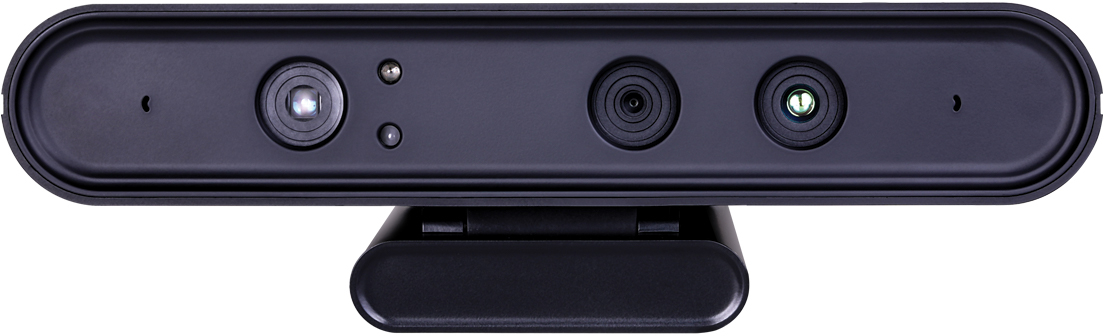
\includegraphics[width=0.6\textwidth]{figs/AstraPro.jpg}}
\caption[Orbbec Astra Pro]{Orbbec Astra Pro \cite{AstraPro}}
\label{fig:orbbec_astra_pro}
\end{figure}

In the experimental setup, one of the cameras is placed above the workspace facing downwards allowing the perception of position of the user's hand through the color and depth images. The second camera is above and slightly behind the robot to capture the user in front of the robot with the images from this camera being the ones used in the keypoint detection models. The communication with the cameras is established through ROS with the $usb\_cam$ package being used for the color image and the $ros\_astra\_camera$ package being used for the depth image.

The camera calibration was done using the $camera\_calibration$\footnote{$camera\_calibration$ package wiki page: \url{https://wiki.ros.org/camera_calibration}} package for the intrinsic parameters and the $atom$\footnote{$atom$ package documentation: \url{https://lardemua.github.io/atom_documentation/}} package for the extrinsic parameters. The calibration process was done by capturing images of two charuco boards placed in the workspace.

\subsection{Manipulator Arm Control}
\label{subsection:manipulator_arm_control}

The collaborative robot available for this work is a UR10e model which was developed by Universal Robots. This model has six degrees of freedom with six rotational joints, allows for payloads up to \SI{12.5}{\kilogram}, and has a reach of \SI{1300}{\milli\metre} being suitable for tasks such as machine tending, palletizing, and packaging\cite{UR10e}. In this work, the robot is equipped with a 2F-140 gripper developed by Robotiq, commonly used together with robot models from Universal Robots\cite{robotiq_gripper}.

\begin{figure}[ht]
    \centerline{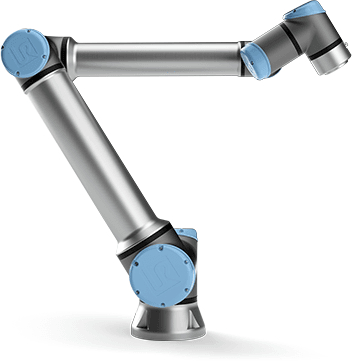
\includegraphics[width=0.4\textwidth]{figs/UR10e.jpg} \ \ 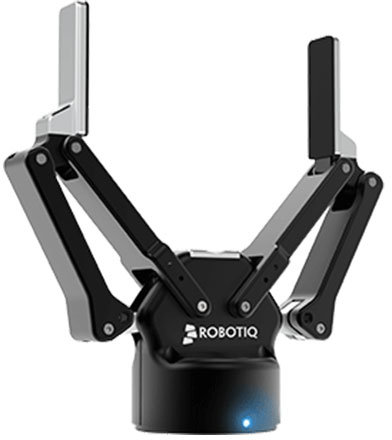
\includegraphics[width=0.35\textwidth]{figs/robotiq-2f-140.jpg}}
    \caption[UR10e Collaborative Robot and Robotiq 2F-140 Gripper]{UR10e Collaborative Robot \cite{UR10e_image} and Robotiq 2F-140 Gripper \cite{robotiq_gripper}}
    \label{fig:ur10e}
\end{figure}

Both the robot and the gripper have ROS packages containing their drivers making their integration easier. The planning and execution of the arm movements are done through the MoveIt\footnote{MoveIt documentation: \url{https://ros-planning.github.io/moveit_tutorials}} framework, which is a widely-used open-source framework for robotics applications involving motion planning, manipulation, 3D perception, kinematics, control, navigation, and collision checking, with OMPL being chosen to handle the motion planning tasks.

The configurations of the drivers and MoveIt was already done by other members of the AUGMANITY project and can be found on Github\footnote{Github LarCC Repository: \url{https://github.com/lardemua/larcc_drivers}} along with a higher-level API that encloses that logic.

In the last part of this work, the $ur\_rtde$\footnote{UR RTDE Documentation: \url{https://sdurobotics.gitlab.io/ur_rtde/index.html}} package was used to control the robot's movements using velocities instead of positions. This package allows to do everything that can be done with teach pendant connected to the robot, such as moving the robot and even turning on and off the free drive mode.

\subsection{Computational Systems}

The tasks involved in this work, such as training deep-learning models and analyzing images in real-time require high computational resources. To handle the real-time processing of images and robot control, the central computer present in the setup was used. To handle the deep-learning model training, the deep-learning research server from LAR was used, codenamed Deeplar:
\begin{itemize}
    \item AMD RyzenTM Threadripper 2950X;
    \item Four NVIDIA GEFORCE® RTX 2080 Ti;
    \item 128GB DDR4 RAM.
\end{itemize}

The model training in Deeplar is executed using docker images, which allows multiple people to use the computer with each having their own isolated training environment with their own dependencies. The images used to design and train machine learning models in this work are based on the latest TensorFlow official image for GPUs.

TensorFlow is one of the most popular machine learning frameworks along with Pytorch. In this work, the former was chosen over the latter since the higher-level API allowed for faster development. The main features of Tensorflow\footnote{Tensorflow documentation: \url{https://www.tensorflow.org/api_docs}} are:
\begin{itemize}
    \item \textbf{prepare data}: load data, data pre-processing and data augmentation;
    \item \textbf{build models}: design and train custom models with little code or use pre-trained ones (transfer learning);
    \item \textbf{deploy models}: helps using models in different platforms such as locally, in the cloud, in a browser, or in mobile;
    \item \textbf{implement MLOps}: run models in production, tracking their performance and identifying issues.
\end{itemize}

\subsection{Keypoints Detection with MediaPipe}
\label{subsection:keypointdetection}

MediaPipe\footnote{MediaPipe documentation: \url{https://developers.google.com/mediapipe}} consists of a set of libraries and tools to apply AI and Machine Learning techniques in other applications, particularly in pipelines for advanced real-time vision-based applications \cite{Lugaresi2019}. Although it contains many features, in this work the focus is on the Hand and the Pose Landmark Detection Models.
The Hand Landmark Detection model \cite{Zhang2020} uses two sub-modules: a hand palm detection model and a hand landmark model. Each frame of an RGB input is fed into the palm detection model, which produces a bounding box based on the palm. The hand landmark model uses this bounding box and returns the keypoint localization of 21 landmarks, including the fingertips, the finger joints (knuckles), and the base of the palm (\autoref{fig:mediapipe_hand_landmarks}). The Pose Landmark Detection model also uses two sub-modules working in a similar way to return 33 landmarks over the entire body (\autoref{fig:mediapipe_pose_landmarks}).

\begin{figure}[ht]
    \centering
    \begin{subfigure}[b]{0.49\textwidth}
        \adjincludegraphics[width=\textwidth, trim={{.15\width} {0} {.05\width} {0}}, clip]{figs/hand_landmarker.jpg}
        \caption{}
        \label{fig:mediapipe_hand_landmarks}
    \end{subfigure} \
    \begin{subfigure}[b]{0.49\textwidth}
        \adjincludegraphics[width=\textwidth, trim={{0} {0} {.20\width} {0}}, clip]{figs/pose_landmarker.jpg}
        \caption{}
        \label{fig:mediapipe_pose_landmarks}
    \end{subfigure}
    \caption[Mediapipe landmarker models: Hand Landmarker and Pose Landmarker.]{Mediapipe landmarker models \cite{mediapipe_docs}: (a) Hand Landmarker and (b) Pose Landmarker.}
    \label{fig:mediapipe_landmarks}
\end{figure}

\subsection{RL Simulator}

\textcolor{red}{Gymnasium and Mujoco}
\section{Learning-Based Recognition of Human-Grasped Objects}

\subsection{Proposed Approach}
\label{subsection:proposal_overview}

% The adopted solution  focuses on detecting and tracking the hand and finger keypoints from visual data. 
This work contains a learning-based framework to enable an assistive robot to recognize the object grasped by the human operator. As illustrated in \autoref{fig:LearningFramework}, it combines the strengths of MediaPipe in detecting hand landmarks in a RGB image with a deep multi-class classifier that predicts the object based on the configuration of the user's hand after grasping it. Accordingly, the developed object recognition system operates based on different principles, including the sensing device, the tracking method, and the machine learning approaches. From the point of view of the application in industrial settings, the proposed system has two strengths when compared to the use of data-gloves or electromagnetic motion capture systems. First, the simplicity of installation is associated with a much less complex and costly setup. Second, the non-intrusiveness of the required setup is a valuable factor in accelerating the acceptance of these technologies by humans in carrying out collaborative tasks (a process also referred to as "user adoption"). In contrast, vision-based hand tracking is affected by occlusions, changes in light conditions, and cluttered backgrounds. Furthermore, these problems are difficult to overcome with deep-learning techniques given the data dependency and generalization problems against hands, objects, and lighting conditions outside the training sets. Overall, this paper contributes to advances in understanding the opportunities and limitations of using this novel approach for the recognition of human-grasped objects.

\begin{figure}[ht]
    \centering
    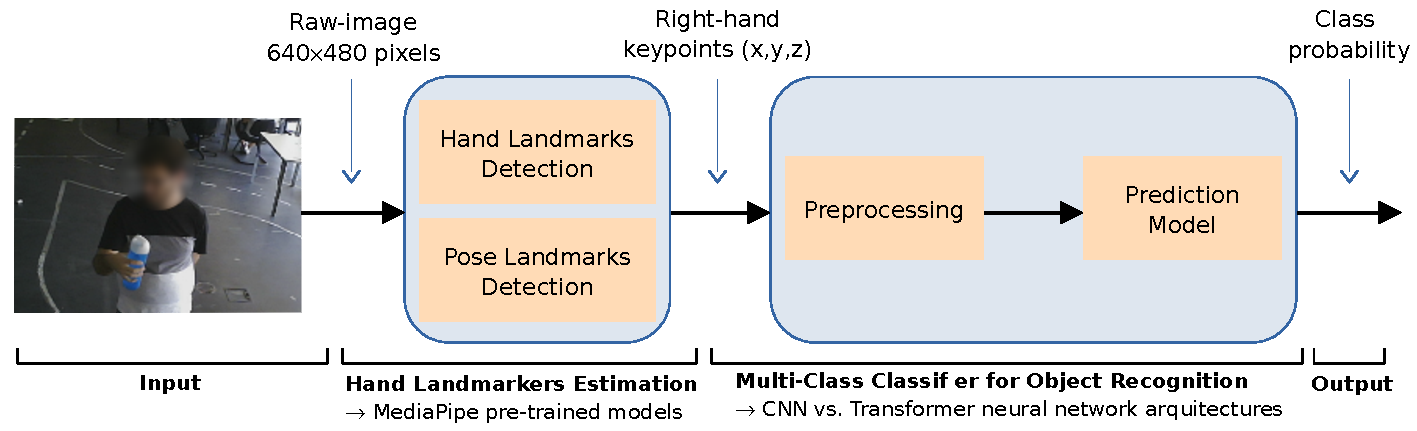
\includegraphics[width=1\columnwidth]{figs/LearningFrameworkB.pdf}
    \caption{The proposed learning-based framework for object recognition based on the hand keypoints.}
    \label{fig:LearningFramework}
\end{figure}

The output of the pre-trained model provides the $(x,y,z)$ coordinates of landmarks for each detected hand. The $(x,y)$ coordinates represent the horizontal and vertical positions of the landmark on the image plane, while the $z$-coordinate represents an estimate of the relative depth with respect to the wrist reference \cite{Amprimo2023}. This work focuses on tracking the right hand by combining the Hand Landmark detection and the Pose Landmark Detection pre-trained models. This strategy proved to be useful to enhance the reliability of the process of extracting the coordinates of the right-hand keypoints from each frame.

The multi-class classifier for object recognition faces several challenges. First, there is limited information about the three-dimensional configuration of the hand, namely if the hand configurations involve overlapping fingers or positions close to each other in the image plane. Consequently, the $z$-coordinate (relative depth) revealed to be a critical element for discriminating complex hand configurations. Second, the coordinates provided by MediaPipe can vary in scale and rotation depending on the hand's distance from the camera and the hand's orientation in the image, adding complexity to the task. For these reasons, a deep learning model able to learn complex features directly from the MediaPipe coordinates will be explored and evaluated with a view to its generalization ability in different scenarios and for various users.

\subsection{Data Representation}
\label{section:data_representation}

The four everyday objects selected for this study are all "graspable", i.e., more or less rigid. They include a cylindrical water bottle, a Rubik's cube, a plier, and a small and sharp screwdriver (\autoref{fig:GraspedObjects}). Given the differences in shape, size, and/or weight, the goal is to discriminate these four objects based on the configuration adopted by the hand while interacting with them.

\begin{figure}[ht]
\captionsetup{width=0.7\textwidth}
\centering
\includegraphics[width=0.7\textwidth]{figs/objects.jpg}
\caption{The objects used in the study include a water bottle, a Rubik's cube, a plier, and a screwdriver.}
\label{fig:GraspedObjects}
\end{figure}

\subsubsection{Dataset Acquisition}

For this particular problem the dataset was manually collected, consisting of videos where one person would move and rotate a particular object (example frames in \autoref{fig:dataset_examples}). This acquisition involved the participation of three right-handed (male) volunteers aged between 23 and 26 years old. Participants were asked to naturally grab and hold an object placed on a table, followed by executing small movements of the hand in free space. These movements were performed while introducing random variations in the hand's orientation relative to the RGB camera to ensure diversity in the points of view from which the hand-object interaction is observed.

\begin{figure}[ht]
    \centerline{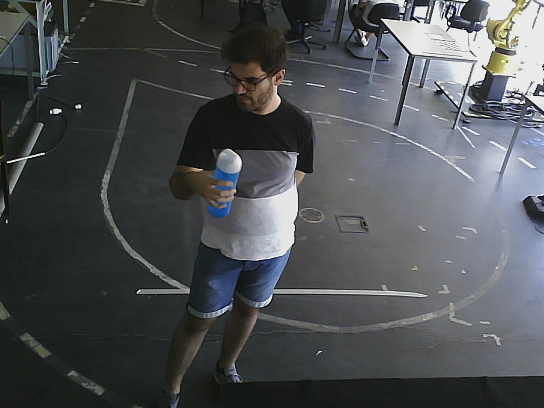
\includegraphics[width=0.4\textwidth]{figs/dataset_preprocessing1_1.png} \ 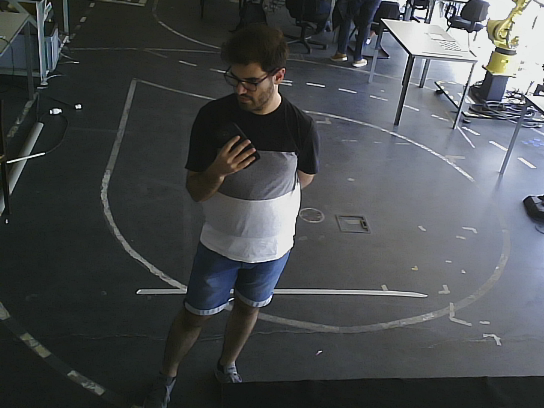
\includegraphics[width=0.4\textwidth]{figs/dataset_preprocessing1_2.png}}
    \caption{Dataset examples holding a bottle (left) and a phone (right).}
    \label{fig:dataset_examples}
\end{figure}

Naturally, the successive frames could lead to similar grasping patterns from different views. To investigate intra-user variability and to ensure robust model training, users are instructed to perform multiple grasping trials of the selected object across four distinct acquisition sessions. Bearing this in mind, the data acquisition system was designed to facilitate the fast generation of training datasets, accommodating the inclusion of new users and/or additional acquisition sessions. On the one hand, the system is integrated into the workflow of the proposed object recognition framework. On the other hand, it is particularly well-suited for implementation in industrial settings where end-users may not possess extensive expertise in machine learning or computer vision. The instructions provided to users during the data acquisition sessions were intentionally straightforward, ensuring that non-experts could readily participate in the process.

Videos over four sessions per user were recorded at 10 frames per second. For each object and each user, four data acquisition sessions were carried out, which gave rise to the dataset used in the study. Therefore, the dataset consists of a total of \num{10229} samples, distributed practically equally across the three participants (around \num{3400} samples per participant) and the four objects (between \num{2166} and \num{2784} samples per object). The exact number of samples of the entire dataset per class and per user is shown in \autoref{tab:dataset}.

\begin{table}[ht] 
\centering
\caption{Number of samples in the dataset per class and user}
\label{tab:dataset}
\begin{tabular}{lccccc}
\toprule
Dataset & Bottle & Cube & Plier & Screwdriver & Total \\
\midrule
User1 & \num{649} & \num{890} & \num{943} & \num{956} & \num{3438}\\
User2 & \num{771} & \num{836} & \num{872} & \num{898} & \num{3377}\\
User3 & \num{746} & \num{834} & \num{904} & \num{930} & \num{3414}\\
\midrule
Total & \num{2166} & \num{2560} & \num{2719} & \num{2784} & \num{10229}\\
\bottomrule
\end{tabular}
\end{table}

\subsubsection{Preprocessing}

After having a dataset, the data had to be processed to have a fitting structure to be used in the model training. The images from the videos were processed using the Mediapipe hands model resulting in 21 points for each hand detected (\autoref{fig:dataset_examples2}).

\begin{figure}[ht]
    \centerline{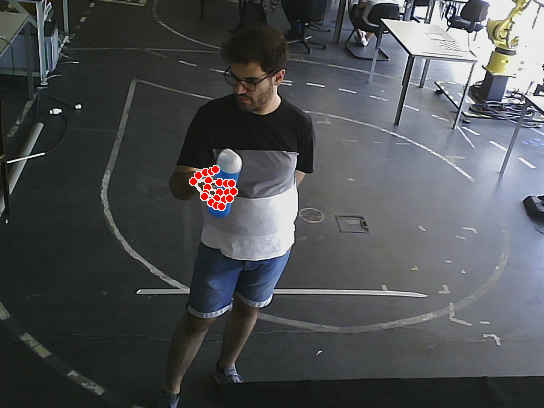
\includegraphics[width=0.4\textwidth]{figs/dataset_preprocessing2_1.png} \ 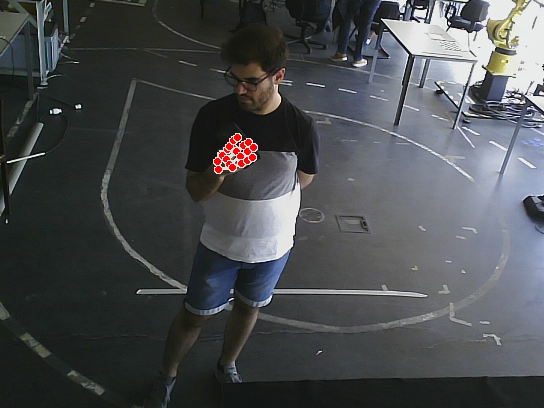
\includegraphics[width=0.4\textwidth]{figs/dataset_preprocessing2_2.png}}
    \caption{Points detected on the pictures in \autoref{fig:dataset_examples} by Mediapipe Hands Model.}
    \label{fig:dataset_examples2}
\end{figure}

The points corresponding to the right hand are then subject to further transformations and normalization. First, the original coordinates of the keypoints (raw data), which are already normalized within the range of 0 to 1 are converted into coordinates relative to a reference. Specifically, for each keypoint $P = (x,y,z)$, the coordinates of the reference point are subtracted $P_{ref} = (x_{ref}, y_{ref}, z_{ref})$ from them to obtain relative coordinates $P_{rel} = (x_{rel}, y_{rel}, z_{rel})$. In this study, the reference is defined as the centroid $C$ of the set of hand keypoints.
This transformation into relative coordinates is particularly useful because the absolute position of the hands in the image may vary from frame to frame due to different distances from the camera or hand orientations. Instead, relative coordinates are translation invariant and they reduce the influence of any rotations that might be present in the raw data. Therefore, the network will focus on the spatial relationships between keypoints, rather than their absolute positions, making it less sensitive to hand orientations and scale variations.

After obtaining the relative coordinates with respect to the reference point, scaling is applied to each dimension independently by dividing by an appropriate constant to ensure that the hand’s representation spans the entire range, as follows:
\begin{equation}
scaleFactor = \frac {0.5}{\max(\{\lvert x_i \rvert,\lvert y_i \rvert,\lvert z_i\rvert\}: i=1,\cdots,n)} \text{  ,}
\end{equation}
%
where $\{x_i,y_i,z_i\}$ denote relative coordinates. This feature scaling revealed to be a valuable pre-processing step to help make the data more consistent, helping the model to learn the relevant patterns without being influenced by variations in hand position, hand size, or scale. Further, it helps to maximize the separation among keypoints, helping the model to discriminate the output class. Finally, a uniform adjustment is made by adding 0.5 to each coordinate, centering the points between 0 and 1 on the scale. It is important to note that throughout the point processing, the order of the points is never changed, and therefore the models can take advantage of this structure. \autoref{fig:dataset_examples3} shows examples of the normalized keypoints representation expressed according to the previous steps, that is: 
\begin{equation}
P_{norm} = (P - C) \times scaleFactor + 0.5\text{ .}
\end{equation}

\begin{figure}[ht]
    \centerline{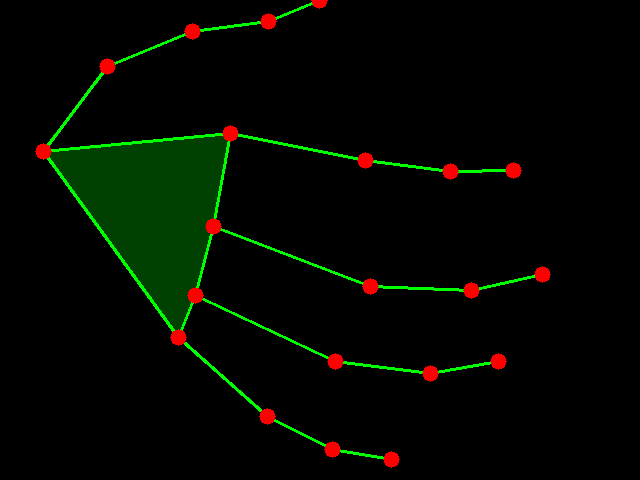
\includegraphics[width=0.4\textwidth]{figs/dataset_preprocessing3_1.png} \ 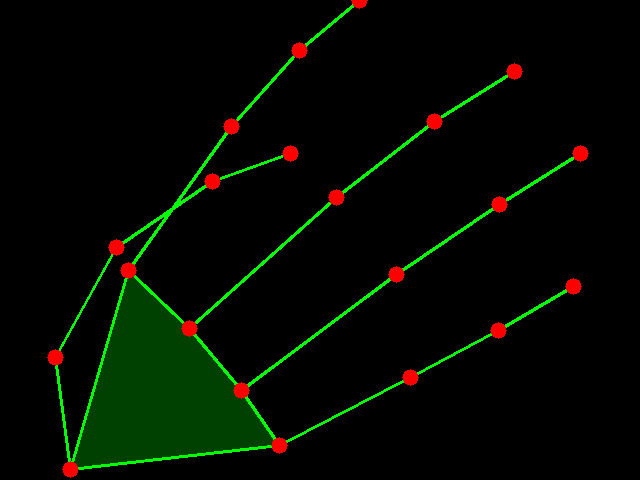
\includegraphics[width=0.4\textwidth]{figs/dataset_preprocessing3_2.png}}
    \caption{Points from the pictures in \autoref{fig:dataset_examples2} after normalization}
    \label{fig:dataset_examples3}
\end{figure}

\subsection{Models}

For this work, the architectures tested were the CNN and the Transformer given their ability at detecting local relations, which makes them an advantageous solution for this problem given that each sample provided to the model is made of the 21 3D points that always follow the same structure representing the right hand. For further details on the models, \textcite{Amaral2023} provides a more in-depth description of the models' training and evaluation.

\subsubsection{CNN Classifier}
\label{subsubsection:cnn_classifier}

The developed CNN comprises two convolutional layers each with 64 feature maps and ReLU activation functions. 
The first layer uses a kernel size of 3$\times$3 pixels performing a 1D convolution on the 3$\times$21 data with a stride of 1 pixel. The flattened output from the final layer is connected to a dense layer with 128 neurons, followed by another dense layer with the number of neurons equal to the number of classes. The output layer consists of the final connect layer with softmax activation. The softmax function takes a vector of real-valued scores (often called logits) and transforms them into a probability distribution over multiple classes. For the classification task with 4 classes, the output layer has 4 neurons, each representing the probability of the input belonging to a particular class. To prevent overfitting, dropout layers are incorporated after each fully connected layer. The final model can be seen in \autoref{fig:cnn_architecture} and it has \num{156644} trainable parameters. It is made of two convolutional layers followed by three dense layers, with the third being the output layer. Between the convolutional and the dense layers and between both dense layers, there is also a dropout layer to help with overfitting.

\begin{figure}[ht]
    \centering
    {\fontsize{9}{11}\selectfont\includesvg[width=\textwidth]{figs/cnn_architecture.svg}}
    \caption{CNN model architecture}
    \label{fig:cnn_architecture}
\end{figure}

\subsubsection{Transformer Neural Network Classifier}
\label{subsubsection:transformer_classifier}

The developed Transformer model is made of two Transformer encoder stacks (\autoref{fig:transformer_encoder_architecture}) comprised of the following layers: multi-head self-attention, layer normalization, and feedforward neural networks. Within each encoder, multi-head self-attention is applied to capture dependencies among the keypoints, where four attention heads are used for enhanced feature extraction. Following self-attention, two position-wise feedforward neural networks are employed to process the attended features and capture complex patterns. Layer normalization is applied after each sub-layer to stabilize the activations and facilitate training convergence. The resulting architecture can be seen in \autoref{fig:transformer_architecture} and it has \num{16384} trainable parameters.

\begin{figure}[H] %[ht]
    \centering
    {\fontsize{10}{12}\selectfont\includesvg[width=1\textwidth]{figs/transformer_encoder.svg}}
    \caption{Transformer encoder block}
    \label{fig:transformer_encoder_architecture}
\end{figure}

\begin{figure}[H] %[ht]
    \centering
    {\fontsize{10}{12}\selectfont\includesvg[width=1\textwidth]{figs/transformer_architecture.svg}}
    \caption{Transformer model architecture}
    \label{fig:transformer_architecture}
\end{figure}

\subsection{Model Comparison}

With both models trained, \autoref{table:model_comparison} shows the performance of all the machine learning models involved in this classification task, including those belonging to MediaPipe.

\begin{table}[H] %[ht]
    \centering
    \caption{Model Comparison}
    \label{table:model_comparison}
    \begin{tabular}{lcc}
        \toprule
        Model & Performance & Prediction Time (ms) \\
        \midrule
        Hand Landmarker & 10.09 MNAE* & 43.5 \\
        Pose Landmarker Lite & 87.0 PDJ* & 21.8 \\
        Pose Landmarker Full & 91.8 PDJ* & 28.7 \\
        Pose Landmarker Heavy & 94.2 PDJ* & 83.1 \\
        CNN Object Classifier & 90.5\% Acc* & 14.1 \\
        Transformer Object Classifier & 86.7\% Acc* & 16.0 \\
        \bottomrule
    \end{tabular}
    \captionsetup{width=0.9\textwidth}
    \caption*{*MNAE: Mean of Normalized Absolute Error\\ *PDJ: average Percentage of Detected Joints\\ *Acc: Accuracy}
\end{table}

For the Hand Landmarker, there is only a single option available so it was the one used. Then, for the Pose Landmarker there are three options available but given that it has relatively less relevance and it runs in parallel with the Hand Landmarker, the Full version was used since it has the highest performance while keeping a lower prediction time. Finally, for the object classifier, the CNN presented the highest accuracy and the lowest prediction time so it was selected for further optimizations in real-time.

With all models of the pipeline selected, a test was made in real-time for each object to check the stability and reliability of the model prediction in a certain frame, resulting in the graphics in \autoref{fig:bottle_softmaxes}, \autoref{fig:cube_softmaxes}, \autoref{fig:plier_softmaxes} and \autoref{fig:screw_softmaxes}.

\begin{figure}[H]
    \centering
    {\fontsize{9}{11}\selectfont\includesvg[width=0.98\textwidth]{figs/bottle_cnn_softmaxes.svg}}
    \caption{Bottle Softmaxes}
    \label{fig:bottle_softmaxes}
\end{figure}

\begin{figure}[H]
    \centering
    {\fontsize{9}{11}\selectfont\includesvg[width=0.98\textwidth]{figs/cube_cnn_softmaxes.svg}}
    \caption{Cube Softmaxes}
    \label{fig:cube_softmaxes}
\end{figure}

\begin{figure}[H]
    \centering
    {\fontsize{9}{11}\selectfont\includesvg[width=0.98\textwidth]{figs/plier_cnn_softmaxes.svg}}
    \caption{Plier Softmaxes}
    \label{fig:plier_softmaxes}
\end{figure}

\begin{figure}[H]
    \centering
    {\fontsize{9}{11}\selectfont\includesvg[width=0.98\textwidth]{figs/screwdriver_cnn_softmaxes.svg}}
    \caption{Screwdriver Softmaxes}
    \label{fig:screw_softmaxes}
\end{figure}

These results show that there are a significant number of frames where the model outputs a softmax probability equal or very close to \num{1.0} about the wrong label, especially in the video where the user is holding a plier. Furthermore, these frames are not isolated, sometimes the error happens over multiple consecutive frames making it even harder to establish a rule about when a prediction is valid.

With the unreliability of the softmax probability, the values of the neural network before the softmax operation names logits were tested to ascertain if they would be able to provide additional information, resulting in the graphics in \autoref{fig:bottle_logits}, \autoref{fig:cube_logits}, \autoref{fig:plier_logits} and \autoref{fig:screw_logits}.

\begin{figure}[H]
    \centering
    {\fontsize{9}{11}\selectfont\includesvg[width=0.98\textwidth]{figs/bottle_cnn_logits.svg}}
    \caption{Bottle Logits}
    \label{fig:bottle_logits}
\end{figure}

\begin{figure}[H]
    \centering
    {\fontsize{9}{11}\selectfont\includesvg[width=0.98\textwidth]{figs/cube_cnn_logits.svg}}
    \caption{Cube Logits}
    \label{fig:cube_logits}
\end{figure}

\begin{figure}[H]
    \centering
    {\fontsize{9}{11}\selectfont\includesvg[width=0.98\textwidth]{figs/plier_cnn_logits.svg}}
    \caption{Plier Logits}
    \label{fig:plier_logits}
\end{figure}

\begin{figure}[H]
    \centering
    {\fontsize{9}{11}\selectfont\includesvg[width=0.98\textwidth]{figs/screwdriver_cnn_logits.svg}}
    \caption{Screwdriver Logits}
    \label{fig:screw_logits}
\end{figure}

The results show that across all four classes, when a logit value is higher than six, the model is always giving a correct prediction for the bottle and cube classes and almost always in the other two. This information can be used to create a rule that will only consider the prediction valid if the highest logit value is higher than six. As an extra layer of security, the prediction will only be considered valid if the model gives the same prediction for two consecutive frames. 

\section{Path Planning using Reinforcement Learning}

\subsection{Environment}

The environment used for model training was based on the Fetch Reach environment made available by Gymnasium Robotics (https://robotics.farama.org/envs/fetch/reach/). In this environment, the task was to make the manipulator move the end-effector to a random 3D position above a table in front of the robot, as show in \autoref{fig:fetch_reach_env}. The robot in this simulation has 7-DoF and is controlled by small displacements of the gripper in cartesian coordinates, with Mujoco being responsible for the inverse kinematics computation.

\begin{figure}[H]%[ht]
    \centerline{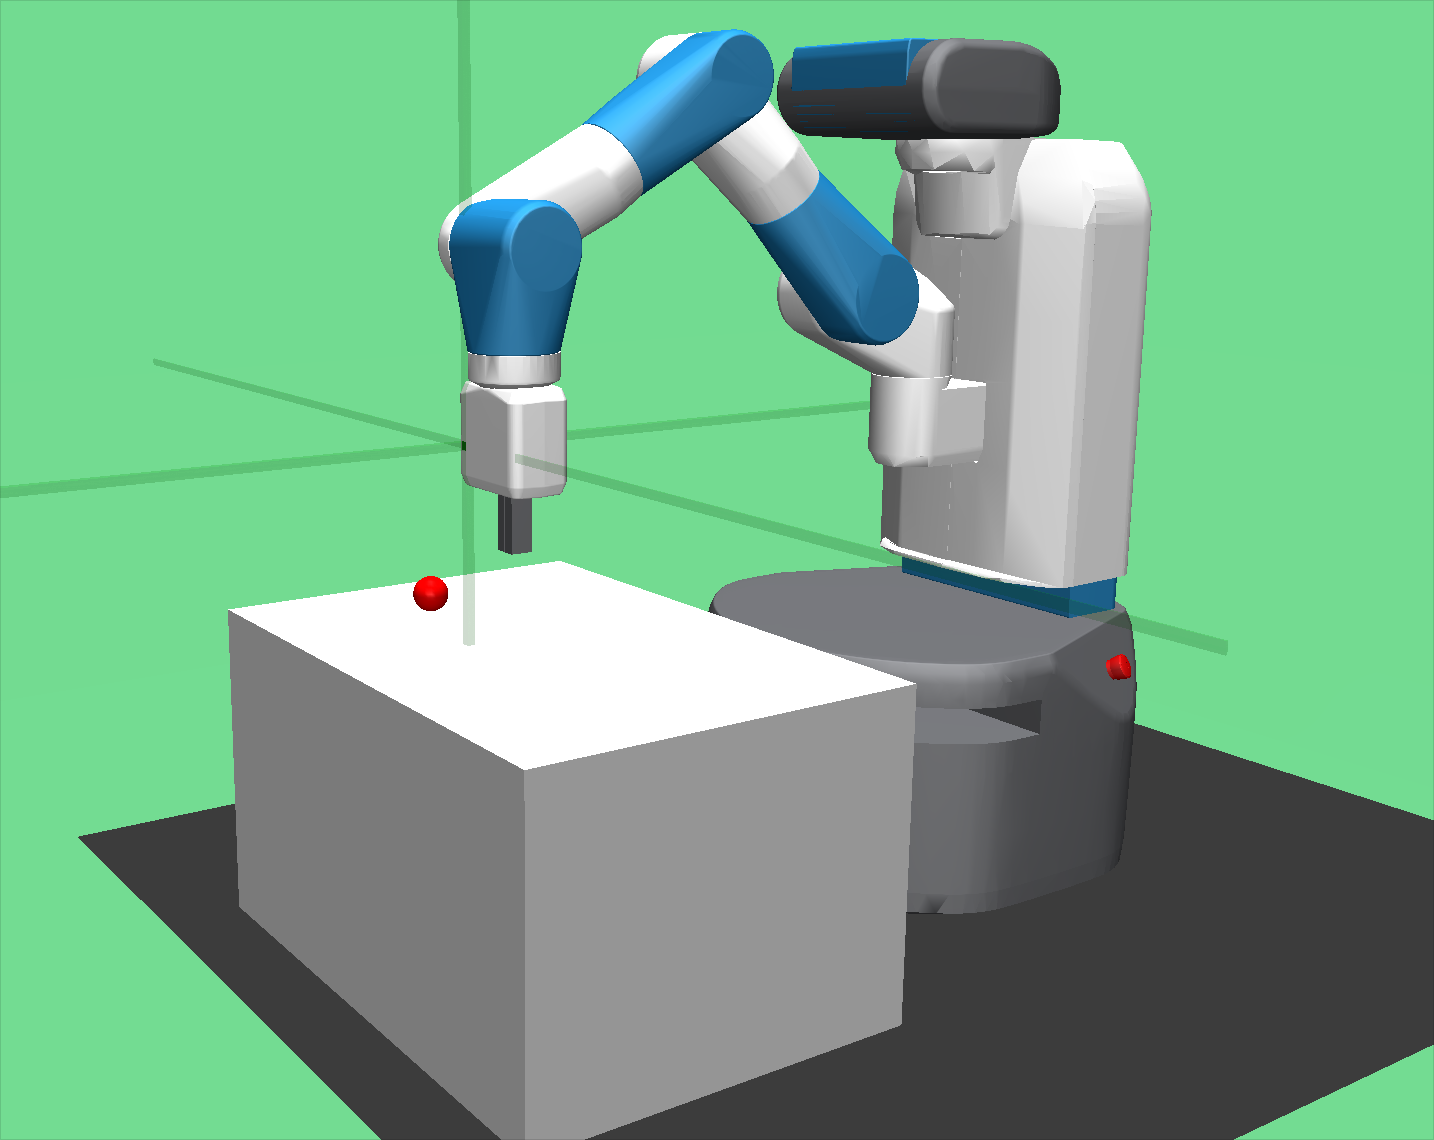
\includegraphics[width=0.7\textwidth]{figs/fetch_reach.png}}
    \caption[Fetch Reach Environment]{Fetch Reach Environment}
    \label{fig:fetch_reach_env}
\end{figure}

The Fetch Reach environment served as a starting point for this research but ended up being mostly rewritten to not only resemble the available collaborative cell but also allow for direct joint control instead of the previous cartesian displacements. The final environment, now named Larcc, can be seen in \autoref{fig:larcc_env} which now includes a UR10e robot model with a Robotiq 2F-140 gripper just like in the real collaborative cell. \textcolor{red}{(should probably refer the sources of the models around here)} The models used were deemed acceptable given that the difference between the end-effector position in ROS and in the simulator differ by less than 1mm for the same joint positions. In this environment, the goal is to move the end-effector to a target position and orientation which are both represented by 3D axes in the simulator. As the actions affect the joints directly, a model trained is this environment ends up replacing the inverse or differential kinematics.

\begin{figure}[H]%[ht]
    \centerline{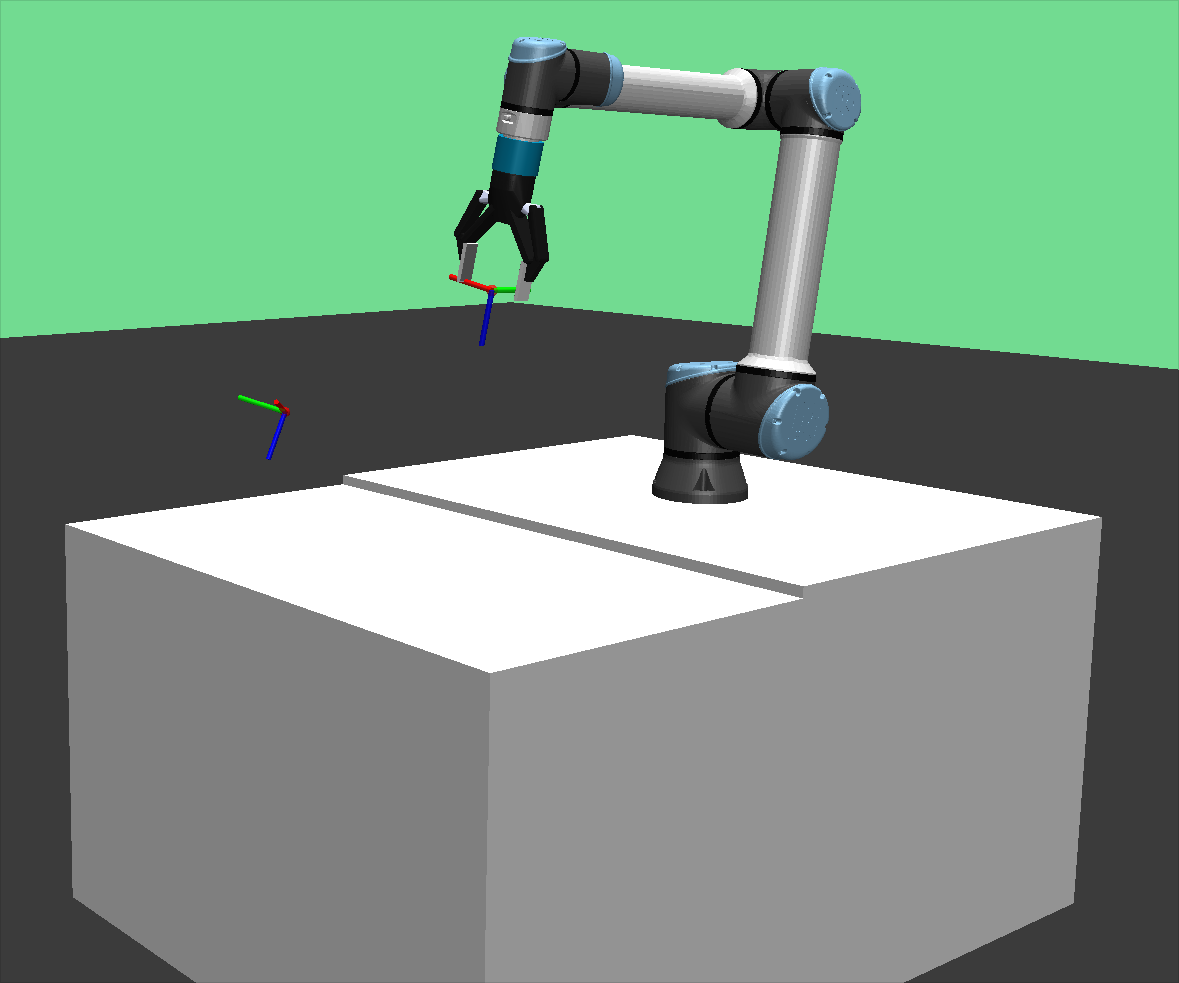
\includegraphics[width=0.7\textwidth]{figs/larcc_env.png}}
    \caption[Larcc Environment]{Larcc Environment}
    \label{fig:larcc_env}
\end{figure}

\subsubsection{Starting State}

To set up a new episode during training, the robot state and the goal position and orientation in the environment are reset.

For the goal, the position is sampled from a uniform distribution corresponding to the volume \SI{10}{\cm} to \SI{60}{\cm} above the table in front of the robot. The orientation is sampled from a uniform distribution in RPY format and then converted to quaternions. The orientation is then validated to check if it is facing mostly forward and downwards, which is the orientation that the gripper should have to pick up an object. If the orientation is not valid, a new one is sampled until a valid one is found.

For the starting state of the robot there are two possibilities: it can start in the fixed position shown in \autoref{fig:larcc_env} or in a random position. The random position is obtained by sampling the joint positions from a uniform distribution in the $[-\pi, \pi]$ interval, which is the same interval used for the joint limits in the UR10e robot. However, given that a fully random starting position can make the task too difficult, the end-effector position and orientation from the random starting position is validated with the same constraints as the goal position and a new starting position is sampled until a valid one is found.

\subsubsection{Observation Space}

The observation space in this environment follows the structure commonly used Gymnasium environments being a dictionary with 3 keys:

\begin{itemize}
    \item $observation$: consists of the positions of the 6 joints; given that they were limited to the $[-\pi, \pi]$ interval, they were normalized by a division by $\pi$;
    \item $achieved\_goal$: current position and orientation of the end-effector; the position was normalized by subtracting the position of the robot base link in the environment and then dividing by the arm's range, and the orientation was kept because it is defined with quaternions which are already in the $[-1, 1]$ interval;
    \item $desired\_goal$: position and orientation of the goal; normalized in the same way as the achived\_goal above.
\end{itemize}

\subsubsection{Action Space}

The action space represents the displacements in all joints for a single timestep. These displacements are also normalized which means that the final action applied to the environment is the result of the action output given by a model which is in the $[-1, 1]$ range multiplied by the maximum displacements of the joints. The first two joints associated with the shoulder can move at most 0.8 radians per timestep while the other four joints associated with the elbow and the wrist can move at most 1.2 radians per timestep, representing the different maximum velocities on the UR10e robot joints (https://www.universal-robots.com/products/ur10-robot/).

\subsubsection{Rewards}

The used environment has dense rewards so as to give the agent frequent and consistent feedback about its actions. This means that in every timestep the reward will increase if the the end-effector is closer to the goal and decrease otherwise, helping the model learn which actions lead to a successful episode. The reward in each timestep is obtained from the following rewards:

\begin{itemize}
    \item $position$: $1-distance(goal\_pos, end$-$effector\_pos)$ if distance lower than 2 otherwise $-1$ so that it is normalized;
    \item $orientation$: $max(innerproduct(goal\_quaternion, end$-$effector\_quaternion), innerproduct(-goal\_quaternion, end$-$effector\_quaternion)$;
    \item $bonus$: $1$ if goal has been reached else $0$; the goal is considered reached if both the other rewards are above $0.98$.
\end{itemize}

These rewards affect the final timestep reward with different weights, but the sum of the weights is always equal to $1$ keeping the final reward in the $[-1, 1]$ range.

\subsection{Soft Actor-Critic (SAC) Model}

\textcolor{blue}{The tests in the described environment were executed using the Soft Actor-Critic (SAC) algorithm. SAC is an off-policy model-free reinforcement learning algorithm that is based on the maximum entropy reinforcement learning framework. This framework allows the agent to learn a policy that maximizes the expected reward while also maximizing the entropy of the policy. This means that the agent will not only try to maximize the reward but also to explore the environment as much as possible. The entropy term in the loss function is weighted by a temperature parameter $\alpha$ which is learned by the model.}

\subsection{Results}

A SAC model was trained on the developed environment with a fixed initial robot state and with a $0.5$ weight on the position reward and a $0.25$ weight on the orientation and on the bonus reward. The model was trained with early stopping configured to evaluate the model every $500$ episodes and stop training if the evaluation average reward does not increase for $20$ evaluations. \autoref{tab:sac_results} shows the results when the best model was saved.

\begin{table}[ht] 
\centering
\caption{SAC Results when the Best Model was Saved}
\label{tab:sac_results}
\begin{tabular}{ccc}
\toprule
\multirow{2}{0.25\textwidth}{\centering Training Episodes} & \multirow{2}{0.25\textwidth}{\centering Training Episode Reward Mean} & \multirow{2}{0.25\textwidth}{\centering Validation Episode Reward Mean} \\
& & \\
\midrule
53500 & 42.9 & 45.3\\
\bottomrule
\end{tabular}
\end{table}

Considering that the maximum reward in a single episode is $50$, the model was able to reach a reward close to the maximum. Additionally, the fact that the validation reward is higher than the training reward is expected given that the in the trainig episodes the model attempts to explore the environment according to its entropy while in the validation episodes the model takes the best actions according to its learned policy.


\section{Robot Controller}
\section{Conclusion}

\color{red}

\section{Plano Inicial de Atividades (To Remove)}

Bolseiro: Pedro Miguel Loureiro Amaral

Orientadores: Filipe Miguel Teixeira Pereira da Silva; Vitor Manuel Ferreira dos Santos

Duração /início e fim do contrato: 6 meses - 16/01/2024 a 15/07/2024

Projeto: UIDB/00127/2020

Centro de custos: 3.62.80.11

Local de trabalho: Instituto de Engenharia Eletrónica e Informática de Aveiro (IEETA)

Título plano de trabalhos: Aprendizagem por reforço para antecipar a intenção humana em tarefas colaborativas

Contexto e objetivo da bolsa: A aprendizagem por reforço oferece uma metodologia para desenvolver políticas que maximizam a eficiência da colaboração humano-robô, levando em consideração as ações e intenções humanas. O plano de atividades visa a integração destas metodologias com ferramentas computacionais desenvolvidos no âmbito do projeto Augmanity (https://www.augmanity.pt). Neste contexto, o objetivo da bolsa está centrado no desenvolvimento de um sistema robótico capaz de antecipar as ações e/ou intenções de um operador humano durante a realização de tarefas colaborativas usando técnicas de aprendizagem por reforço, tendo em vista melhorar a eficiência e a segurança dos parceiros envolvidos.

Tarefas a desenvolver:

T1.Tarefa 1 - Levantamento do estado atual de conhecimento das tecnologias e metodologias associadas à capacidade de antecipação em robótica colaborativa.

T2.Tarefa 2 - Desenvolvimento de uma solução integrada baseada em técnicas de aprendizagem por reforço que permitam a um robô melhorar as suas capacidades para anticipar as ações e/ou intenções humanas.

T3.Tarefa 3 - Teste e avaliação de vários algoritmos de aprendizagem por reforço aplicados em diferentes cenários em ambientes reais.

T4.Tarefa 4 - Escrita de documentação relevante e preparação de um protótipo demonstrador.

\color{black}

\textcolor{red}{Where should I describe the hand following?}

\begingroup
\renewcommand{\bibfont}{\footnotesize}
% Redefine References name to Portuguese
% Change if you are using english
\defbibheading{bibliography}[References]{
	\section{#1}
}
\setlength\bibitemsep{8pt}
\printbibliography[heading=bibliography]
\endgroup

\end{document}
